\documentclass{article}

\usepackage{epsfig}
\usepackage{graphicx}
\usepackage{listings}
\usepackage{a4wide}
\usepackage[latin1]{inputenc}
%\usepackage[portuges]{babel}
\usepackage[brazil]{babel}
\usepackage{float}

\title{Programa��o V \\ \small{\textbf{Prof. Alan}} \\ \scriptsize{\textbf{alanpedros@yahoo.com.br}}\\
Expression Language (EL ) com JSLT 1.1 e Banco de Dados\\}

\begin{document}

\maketitle

\begin{description}

\item 1 - Crie uma \emph{aplica��o web} no tomcat chamado \emph{BancoDeDados01}, seguindo os
seguintes procedimentos b�sicos:

\begin{enumerate}

\item Criar uma pasta chamada \emph{BancoDeDados01}, dentro da pasta
$C:\setminus Tomcat\setminus webapps$

\item Criar uma pasta chamada \emph{WEB-INF}, dentro da pasta
$C:\setminus Tomcat\setminus webapps\setminus BancoDeDados01$

\item Criar uma pasta chamada \emph{classes}, dentro da pasta
$C:\setminus Tomcat\setminus webapps\setminus
BancoDeDados01\setminus WEB-INF$

\item Criar uma pasta chamada \emph{lib}, dentro da pasta
$C:\setminus Tomcat\setminus webapps\setminus
BancoDeDados01\setminus WEB-INF$ e ponha as bibliotecas
\emph{C:$\setminus$Tomcat$\setminus$webapps$\setminus$jsp-examples$\setminus$WEB-INF$\setminus$lib$\setminus$jstl.jar}
e
\emph{C:$\setminus$Tomcat$\setminus$webapps$\setminus$jsp-examples$\setminus$WEB-INF$\setminus$lib$\setminus$standard.jar}



\end{enumerate}


\item 2 - Crie um projeto no eclipse, chamado \emph{TesteBD01}, em seguida, fa�a os seguintes procedimentos:

\begin{enumerate}

\item Crie uma pasta do tipo \emph{Source Folder}, chamado
\emph{src};

\item Dentro da pasta \emph{src} do item 1, crie um pacote chamado \emph{model}.

\item Dentro da pasta \emph{src} do item 1, crie um pacote chamado \emph{web}.

\item Crie uma pasta \emph{lib}, e ponha a biblioteca
\emph{C:$\setminus$Tomcat$\setminus$common$\setminus$lib$\setminus$servlet-api.jar}
dentro da pasta. Em seguida, dentro do eclipse, clique com o bot�o
direito do mouse em cima do arquivo \emph{servlet-api.jar}, clique
em \emph{Build Path}$\longrightarrow$\emph{Add to Build Path};

\item Implemente sa classes abaixo abaixo:

\begin{verbatim}
package model;

import java.util.Date;

public class Aluno {
    private int id;
    private String nome;
    private String endereco;
    private String telefone;
    private String cpf;
    private Date dtNascimento;
    private float altura;

    protected Aluno(int id, String nome, String endereco, String telefone,
            String cpf, Date dtNascimento, float altura) {
        this.id = id;
        this.nome = nome;
        this.endereco = endereco;
        this.telefone = telefone;
        this.cpf = cpf;
        this.dtNascimento = dtNascimento;
        this.altura = altura;
    }

    public float getAltura() {
        return altura;
    }

    public String getCpf() {
        return cpf;
    }

    public Date getDtNascimento() {
        return dtNascimento;
    }

    public String getEndereco() {
        return endereco;
    }

    public int getId() {
        return id;
    }

    public String getNome() {
        return nome;
    }

    public String getTelefone() {
        return telefone;
    }

}
\end{verbatim}

-------------------------------------------------------------------------------------------------------------------------

\begin{verbatim}
package model;

import java.sql.Connection; import java.sql.DriverManager; import
java.sql.ResultSet; import java.sql.SQLException; import
java.sql.Statement; import java.util.Vector;

public class BancoDeDados {
    private String driver = "sun.jdbc.odbc.JdbcOdbcDriver";
    private String url = "jdbc:odbc:testebanco";
    private String username = "";
    private String password = "";
    private String query = "select * from aluno";

    private Connection connection;
    private Statement statement;

    public BancoDeDados() throws SQLException, ClassNotFoundException{
        Class.forName(this.driver);
        this.connection = DriverManager.getConnection(url,username,password);
        this.statement = connection.createStatement();
    }

    public Aluno[] getAlunos(){
        try{
            ResultSet resultSet = this.statement.executeQuery(this.query);
            Vector<Aluno> vetor = new Vector<Aluno>();
            while (resultSet.next()){
                vetor.add(new Aluno(resultSet.getInt(1),resultSet.getString(2),
                resultSet.getString(3),resultSet.getString(4),
                resultSet.getString(5),resultSet.getDate(6),
                resultSet.getFloat(7)));
            }
            return (Aluno[])vetor.toArray(new Aluno[vetor.size()]);
        }catch(SQLException e){
            return null;
        }
    }

    public void close() throws SQLException{
        this.connection.close();
    }
}
\end{verbatim}
-------------------------------------------------------------------------------------------------------------------------

\begin{verbatim}
package web;

import java.io.IOException; import java.sql.SQLException;

import javax.servlet.RequestDispatcher; import
javax.servlet.ServletException; import
javax.servlet.http.HttpServlet; import
javax.servlet.http.HttpServletRequest; import
javax.servlet.http.HttpServletResponse; import
javax.servlet.http.HttpSession; import javax.swing.JOptionPane;

import model.Aluno; import model.BancoDeDados;

public class RecebeRequisicao extends HttpServlet {

    public void doGet(HttpServletRequest request, HttpServletResponse response)
            throws IOException, ServletException {
        try{
            BancoDeDados bancoDeDados = new BancoDeDados();
            Aluno[] alunos = bancoDeDados.getAlunos();
            request.setAttribute("alunos",alunos);
            RequestDispatcher dispatcher =
            request.getRequestDispatcher("/WEB-INF/exibirdados.jsp");
            dispatcher.forward(request,response);
        }catch(SQLException e){
            HttpSession session = request.getSession();
            session.setAttribute("erro",e.getMessage());
            response.sendRedirect("erro.jsp");
        }catch(ClassNotFoundException e){
            HttpSession session = request.getSession();
            session.setAttribute("erro",e.getMessage());
            response.sendRedirect("erro.jsp");
        }
    }


    public void doPost(HttpServletRequest request, HttpServletResponse response)
    throws IOException, ServletException {
        response.sendRedirect("erro.jsp");
    }
}

\end{verbatim}

\end{enumerate}

\item 3 - Implemente o arquivo ``erro.jsp'' abaixo, e salve na pasta $C:\setminus Tomcat\setminus webapps\setminus BancoDeDados01$:
\begin{verbatim}
<HTML>
 <HEAD>
  <TITLE> Erro </TITLE>
 </HEAD>
 <BODY>
  Erro
 </BODY>
</HTML>
\end{verbatim}

\item 4 - Implemente o arquivo ``exibirdados.jsp'' abaixo, e salve na pasta $C:\setminus Tomcat\setminus webapps\setminus BancoDeDados01\setminus WEB-INF$:
\begin{verbatim}
<%@ taglib prefix="c" uri="http://java.sun.com/jsp/jstl/core" %>

<HTML>
 <HEAD>
  <TITLE> Exibindo Dados </TITLE>
 </HEAD>
 <BODY>
 <center>
<c:forEach var="aluno" items="${alunos}">
----------------------------------------------
 <TABLE>
 <TR>
    <TD>Nome: ${aluno.nome}</TD>
 </TR>
 <TR>
    <TD>CPF: ${aluno.cpf}</TD>
 </TR>
 <TR>
    <TD>Endereco: ${aluno.endereco}</TD>
 </TR>
 <TR>
    <TD>Telefone: ${aluno.telefone}</TD>
 </TR>
 <TR>
    <TD>Data de Nascimento: ${aluno.dtNascimento}</TD>
 </TR>

 <TR>
    <TD>Altura: ${aluno.altura}</TD>
 </TR>
 </TABLE>
</c:forEach>

 </BODY>
</HTML>
\end{verbatim}

\item 5 - Crie o arquivo ``web.xml'' conforme abaixo, e ponha na
pasta $C:\setminus Tomcat\setminus webapps\setminus
BancoDeDados01\setminus WEB-INF$

\begin{verbatim}
<web-app xmlns="http://java.sun.com/xml/ns/j2ee"
    xmlns:xsi="http://www.w3.org/2001/XMLSchema-instance"
    xsi:schemaLocation="http://java.sun.com/xml/ns/j2ee _
    http://java.sun.com/xml/ns/j2ee/web-app_2_4.xsd"
    version="2.4">


<servlet>
    <servlet-name>RecebeRequisicao</servlet-name>
    <servlet-class>web.RecebeRequisicao</servlet-class>
</servlet>

<servlet-mapping>
    <servlet-name>RecebeRequisicao</servlet-name>
    <url-pattern>/TratarRequisicao</url-pattern>
</servlet-mapping>

</web-app>
\end{verbatim}

\item 6 - Copie tudo que estiver na pasta \emph{bin} do projeto criado no eclipse e
ponha na pasta $C:\setminus Tomcat\setminus webapps\setminus
BancoDeDados01\setminus WEB-INF\setminus classes$

\item 7 - Crie um banco de dados no access, com uma tabela aluno conforme abaixo, e depois crie um
odbc chamado testebanco para acess�-lo. Insira tr�s registros da
tabela aluno.

\begin{figure}[ht]
    \centering
    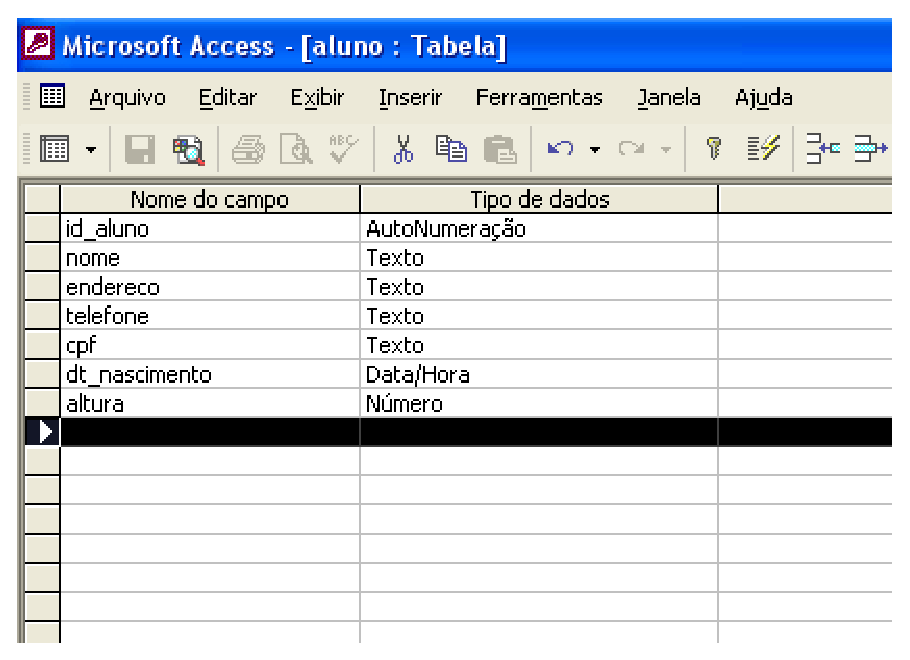
\includegraphics[scale=0.55]{teste.eps}
    \label{img:algoritmoFaratim}
\end{figure}

\item 8 - Reinicie o Tomcat ( $C:\setminus Tomcat\setminus bin\setminus classes\setminus tomcat5$);

\item 9 - Chame a p�gina inicial ( \textbf{http:$//$localhost:8083$/$BancoDeDados01$/$} )
\end{description}

\end{document}
